%\documentclass[pdftex,a4paper,12pt]{article}
\documentclass[pdftex,a4paper,10.5pt]{article}

%\usepackage{graphicx}
\usepackage{float}
\usepackage[pdftex]{graphicx}
%\usepackage[latin1]{inputenc}
\usepackage[spanish]{babel}

\pretolerance=2000
\tolerance=3000

\title{\textbf{Reconocimiento de Figuras Utilizando Redes Neuronales }\\
\begin{normalsize}75.70 - Facultad de Ingenier\'ia de la Universidad de Buenos Aires\end{normalsize} }

%\author{ \textbf{Facultad de Ingenier\'ia de la Universidad de Buenos Aires}\\
%\textbf{75.70} \\ \\ 
%Ciancio Alessio, Mauro -% \textit{Padr\'on Nro. 86.357} \\
%\texttt{maurociancio@gmail.com} \\
%Gilioli, Leandro E. -% \textit{Padr\'on Nro. 86.075} \\
%\texttt{legilioli@gmail.com} \\
%L\'opez El\'ias, Lucas -% \textit{Padr\'on Nro. 85.747} \\
%\texttt{lucasdle@gmail.com} \\
%Ucciani, Juan - %\textit{Padr\'on Nro. 86.473} \\
%\texttt{jucciani@gmail.com} \\
%\texttt{njytito@gmail.com} \\
%\texttt{\{maurociancio,legilioli,lucasdle,jucciani,njytito\}@gmail.com} \\[2.5ex]
%}

\author{
	Ciancio Alessio, Mauro \and
	Gilioli, Leandro E. \and
	L\'opez El\'ias, Lucas \and
	Ucciani, Juan Manuel \and
	Yoan, Norberto \\
	\texttt{\{maurociancio,legilioli,lucasdle,jucciani,njytito\}@gmail.com}
	}
	
\date{1er Cuatrimestre de 2010}


\begin{document}
\maketitle

\begin{abstract}
	Desarrollo de una aplicaci\'on de reconocimiento de figuras a partir del uso y entrenamiento de redes neuronales. Involucra un an\'alisis previo de las figuras cuyo objetivo es extraer de las mimas datos que permitan representarlas adecuadamente para luego reconocerlas por medio una red neuronal.
	
	Se entrena la red neuronal con figuras conocidas. Luego cuando la red est\'a en producci\'on las salidas obtenidas al introducir los datos preprocesados indican el tipo de figura que se reconoci\'o.
\end{abstract}

\thispagestyle{empty}
%\newpage
%\tableofcontents
%\newpage

\section{Introducci\'on}
El presente trabajo utiliza redes neuronales para la detecci\'on de figuras geom\'etricas. 
La aplicaci\'on desarrollada toma una imagen que contiene figuras (cuadrados, tri\'angulos y c\'irculos), y procesa la misma para lograr la normalizaci\'on de los datos con la finalidad de obtener entradas para la red neuronal. 
Una vez procesados los datos de entrada que representan a las figuras de la imagen, la red detecta el tipo de figura.


\section{Desarrollo}
El presente trabajo se encuentra organizado en las siguientes secciones:
\textit{Estado del arte} nos da una idea de las t\'ecnicas actuales utilizadas en aplicaciones similares en el ámbito de detecci\'on de figuras. 
\textit{Presentaci\'on del Problema} presenta el dilema a resolver.
\textit{Resoluci\'on} muestra la definici\'on de la soluci\'on planteada para resolver el problema anterior. 
\textit{Resultados} muestra luego de aplicar la soluci\'on a un conjunto de entradas que representa al espectro de entradas posibles, las diferentes salidas de la aplicaci\'on desarrollada.
Finalmente la secci\'on \textit{Conclusiones} muestra el resultado del an\'alisis del funcionamiento de la aplicaci\'on.

\subsection{Estado del arte \cite{campilho}}
El reconocimiento de formas es un problema central del \'area de visi\'on rob\'otica. Las figuras geom\'etricas pueden ser definidas como contornos de objetos o dominios conectados acotados en el plano. La mayor\'ia de los  m\'etodos de reconocimiento de formas son globales en el sentido de que las caracter\'isticas extra\'idas son calculadas sobre la totalidad de la forma. Las caracter\'isticas globales son en general escalares calculados sobre la totalidad de la figura. Dos caracter\'isticas o discriminantes cl\'asicos se basan en \textit{descriptores de Fourier}\cite{fourierdescriptors} o \textit{momentos invariantes}. Algunos invariantes afines escalares para la representaci\'on global de figuras se pueden derivar de \textit{coeficientes wavelet}. Respresentaciones en el espacio escalar tambi\'en pueden derivarse de representaciones invariantes. En esta clase de m\'etodos el de la \textit{Curvatura del Espacio Escalar}\cite{curvaturescale} es uno de los m\'as populares. \'Estos m\'etodos tratan con el reconocimiento de figuras similares con respecto a la invarianza geom\'etrica. (se buscan figuras similares mediante transformaciones afines por ej.). Por otro lado, un conocido m\'etodo global realacionado con el momento que trata con la similaridad perceptual es el \textit{modal-matching}. En el mismo, las figuras s\'olidas son representadas por \textit{eigenmodes} o \textit{modos propios} asociados a un modelo f\'isico de elasticidad.
 %estado de la cuestin
%[FUMARse gugle e ieee]

\subsection{Presentaci\'on del Problema}
El problema principal que se intenta resolver es reconocer que tipo de figura se encuentra presente en una imagen digital mediante el uso de una red neuronal. Deben poder identificarse correctamente cuadrados, tri\'angulos y c\'irculos. De este problema deriva uno secundario que consiste en procesar adecuadamente la imagen para obtener datos normalizados que sean apropiados para utilizar en la red neuronal. Adem\'as, se deber\'a realizar un entrenamiento de la misma, ajust\'andola de manera que los resultados obtenidos demuestren que se logra la generalizaci\'on de los casos presentados. Se intentar\'a lograr el reconocimiento tanto de figuras que est\'en claramente definidas como tambi\'en de casos en los cuales haya deformaciones o se pueda dar lugar a confusi\'on.


\subsection{Resoluci\'on}
Se encar\'o el problema dividi\'endolo en dos m\'odulos.
\begin{itemize}
\item 
M\'odulo de representaci\'on \cite{rulot}: obtiene, a partir de la imagen provista, una representaci\'on conveniente para su utilizaci\'on por el segundo m\'odulo. La tarea que realiza es el an\'alisis de la imagen de entrada en busca de blobs \cite{blobs} que luego son representados por medio de pol\'igonos de los cuales se extrae informaci\'on caracter\'istica de inter\'es que ser\'a luego alimentada al m\'odulo de la siguiente etapa.
\item
M\'odulo de interpretaci\'on \cite{rulot}: proporciona a partir del conjunto de formas u objetos presentes en la imagen y la representaci\'on convenientemente proporcionada por el m\'odulo de representaci\'on, la forma a la que pertenece el objeto, distinguiendo entre 3 posibles casos: cuadrado, tri\'angulo o c\'irculo.
\end{itemize}



Los pasos realizados por estos m\'odulos se explican a continuaci\'on:

\subsubsection{Pasos}
Para la detecci\'on de las figuras, se realiza el siguiente procedimiento:
			\begin{enumerate}
			  	\item	Se carga en memoria una imagen del archivo que se pasa como 1er
			  	argumento por l\'inea de comando. La aplicaci\'on soporta los formatos m\'as
			  	comunes (png, jpg, bmp, gif).
				\item	Se convierte la imagen a una escala de grises.
				\item 	A partir de la imagen transformada a escala de grises, se hace una
				detecci\'on de los blobs. En este paso se le especifica un umbral para el
				proceso de detecci\'on.
				\item	Se filtran los blobs detectados segun el \'area de la figura.
				\item	Con los blobs resultantes se obtienen los datos que se introducir\'an
				en la red neuronal ($ s_{1}, s_{2}, s_{3} $). Estos datos se denominan \textit{discriminantes basados en caracter\'isticas geom\'etricas} \cite{yangGillies} , y se obtienen a partir de 				           		caracter\'isticas de los blobs:
					\begin{itemize}
                      \item	Distancias promedio al punto central de los v\'ertices
                      del pol\'igono que definen al blob. Se normalizan
                      dividiendo esta distancia por la distancia al v\'ertice m\'as
                      alejado.
                      
  					  \begin{equation} s_{1} = \frac { \sum_{i=1}^{n} { {|\vec {x}_{i} - \vec{x}_{c}|^{2}} } }
				      { \max ( {|\vec{x}_{1} - x_{c}|^{2}}, ... , {|\vec{x}_{n} - \vec{x}_{c}|^{2}} ) }		\end{equation}

					  $ \vec{x}_{i}:  $	 \textit{i-\'esimo punto del pol\'igono. }
					  
					  $ \vec{x}_{c}:  $	 \textit{centroide del pol\'igono. }
						
                      \item	\'Area del pol\'igono que define el blob dividido el 
                      \'area del rect\'angulo de \'area m\'inima que contiene a ese blob.
                      
  					  \begin{equation} s_{2} = \frac { Area Blob }
				                      { Area R_{m}}		\end{equation}

					  $ R{m}:  $	 \textit{ Rect\'angulo de \'area m\'inima que contiene al Blob. }

                      \item N\'umero de v\'ertices del pol\'igono simplificado que
                      define al blob. Cuando se detecta un blob, se le pide a la
                      biblioteca utilizada un pol\'igono que define a ese blob
                      (una lista de puntos x,y). El problema que surge es que
                      esa lista contiene muchos puntos que pueden ser considerados redundantes,
                      por lo que se aplica un algoritmo \cite{ramerDouglas} para la
                      reducci\'on de los mismos que elimina los puntos que no son
                      necesarios sin deformar al pol\'igono.
                      
  					  \begin{equation} s_{3} = \frac { \#Vertices }
				                      { K  }		\end{equation}

					  $ K:  $	 \textit{M\'axima cantidad de v\'ertices para un pol\'igono simplificado. }
                      
 					\end{itemize} 
				\item   Una vez obtenidos los datos, estos son ingresados a la red neuronal
				que posee 3 neuronas de salida.
				\item La neurona que produzca el mayor valor a la salida de la red neuronal corresponde
				al tipo de figura ingresada.

            \end{enumerate}      

Se utiliz\'o una red neuronal del tipo feed-forward entrenada con back-propagation \cite{martinez}. La implementaci\'on utilizada es la que brinda la biblioteca FANN[3]. La topolog\'ia consiste en una capa de entrada con 3 neuronas, una capa oculta con 6 neuronas y una capa de salida con 3 neuronas. Estos valores fueron  definidos luego de realizar varias pruebas con diferentes topolog\'ias posibles y ver que se obten\'ia 
un buen grado de generalizaci\'on con un n\'umero reducido de neuronas. La funci\'on de activaci\'on 
elegida fue una sigmoidal.

El entrenamiento se realiza ajustando continuamente los pesos de manera que 
la salida de la red  concuerde con la salida especificada en el archivo de entrenamiento. Para 
determinar en que nivel la red se ajusta a los resultados deseados, se utiliza el cuadrado de la media 
del error, es decir, el promedio del cuadrado de la diferencia entre la salida actual y la buscada para
cada uno de los casos de entrenamiento. El ciclo se detiene cuando este valor es menor al especificado
al crear la red. Dicho par\'ametro fue probado con valores de 0.01 y 0.001, resultando este \'ultimo el 
elegido por arrojar los mejores resultados.

Para el entrenamiento de la red se utilizaron 15 casos provenientes de una imagen con 15 figuras especialmente seleccionadas para intentar cubrir un buen espectro de posibles casos.
   
             \begin{figure}[H]
	                  \begin{center}
	                    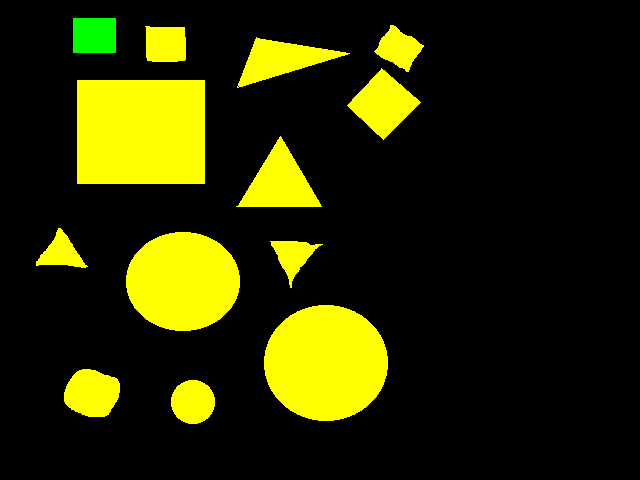
\includegraphics[width=5cm]{prueba2.png}
	                    \caption{\label{entrenamiento} Figuras utilizadas para el entrenamiento. }
	                  \end{center}
	            \end{figure}


%\includegraphics{Screenshot.png}

%incluir imagen de las figuras utilizadas para entrenar la red y quizas una tabla con los valores obtenidos

\subsubsection{Bibliotecas}
La Bibliotecas utilizadas para el desarrollo de la aplicaci\'on son las
siguientes:
\begin{itemize}
	\item	OpenCV \cite{openCV,openCVBook} : Biblioteca open source para el procesamiento de im\'agenes.
	Provee funcionalidad para manipular, transformar im\'agenes, y manejar ventanas de forma sencilla.
	\item	CvBlobs \cite{cvBlob}: Utiliza OpenCV de base y agrega funcionalidad para
	detectar blobs. Permite extraer informaci\'on de inter\'es sobre los mismos, como pol\'igonos que los 
	defienen, \'area y centroide entre otros.
	\item	FANN \cite{fann}: Fast Artificial Neural Network, es una biblioteca open source
	que implementa redes neuronales, entre ellas la de tipo feed-forward y permite realizar el entrenamiento      	de la misma almacenando los resultados y la configuraci\'on en un archivo para su posterior
	utilizaci\'on.
\end{itemize}
       

\subsection{Resultados} %resultados

Luego del proceso de entrenamiento de la red, se gener\'o una imagen con 27 figuras para probar el funcionamiento de la aplicaci\'on. Estas figuras presentan tama\~nos, orientaciones y geometr\'ias diversas para evaluar el grado de generalizaci\'on alcanzado.

En la figura \ref{salida_ejemlpo} se puede apreciar la salida de la aplicaci\'on en la cual puede verse el correcto funcionamiento de la misma en la gran mayor\'ia de los casos.

 	           \begin{figure}[H]

	                  \begin{center}
	                %	\advance\leftskip-1.5cm
	                    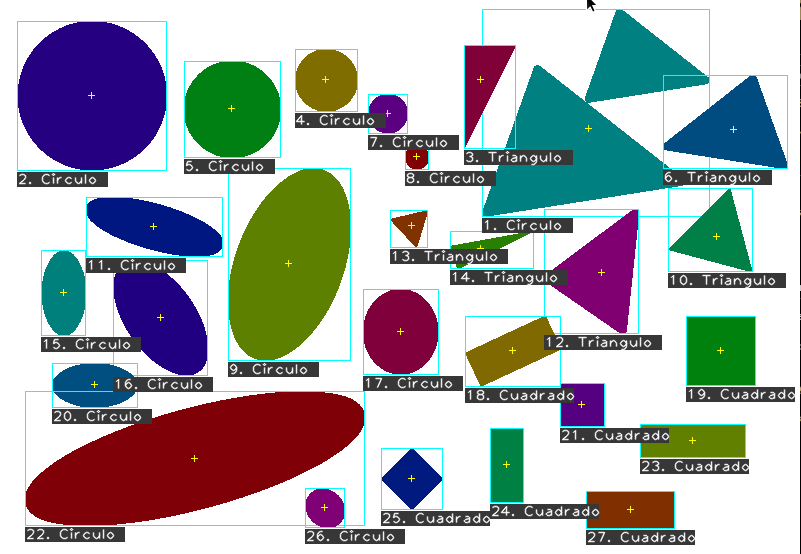
\includegraphics[width=12cm]{salida.png}
	                    \caption{\label{salida_ejemlpo} Salida generada por la aplicaci\'on. }
	                  \end{center}
	            \end{figure}

%\newpage

En la siguiente tabla se pueden apreciar algunos de los datos de entrada y salida de la red neuronal aplicada al caso de prueba presentado.

\begin{table}[ht]
\centering
\begin{tabular}{|l|c|c|c|c|c|c|c|}
  \hline                       
  \textbf{Figura} & \textbf{s1} & \textbf{s2} & \textbf{s3} & \textbf{o1} & \textbf{o2} & \textbf{o3}\\
  \hline
1 & 0.090 & 0.502 & 0.429 & -0.401 & 0.875 & 0.882\\
\hline
3 & 0.030 & 0.525 & 0.299 & 0.000 & 0.964 & -0.020\\
\hline
17 & 0.110 & 0.849 & 0.869 & -0.252 & 0.098 & 0.984\\
\hline
18 & 0.040 & 1.000 & 0.568 & 0.881 & -0.035 & 0.019\\
\hline
19 & 0.040 & 1.000 & 1.000 & 0.911 & 0.010 & 0.011\\

\hline
\end{tabular}	 
\caption{Resultados obtenidos en la corrida de prueba.}
\end{table}

\begin{flushleft}
  $ s_{i}:  $	 \textit{ Entrada de la neurona n\'umero i de la capa de entrada.}\\
  $ o_{i}:  $	 \textit{ Salida de la neurona n\'umero i de la capa de salida. }\\
  $ o_{1}:  $	 \textit{ Corresponde a un cuadrado.}\\
  $ o_{2}:  $	 \textit{ Corresponde a un tri\'angulo.}\\
  $ o_{3}:  $	 \textit{ Corresponde a un c\'irculo.}\\
\end{flushleft}

	        

\newpage
\subsection{Conclusiones} %conclusiones

	En base a los resultados obtenidos, al proceso de desarrollo de la aplicaci\'on y
	entrenamiento de la red podemos elaborar las siguientes conclusiones:
	
	La preparaci\'on de los datos result\'o ser la tarea de mayor complejidad y clave para
	lograr buenos resultados en el reconocimiento. Esto incluye la definici\'on de los atributos
	discriminantes que permitan distinguir a la red entre los distintos tipos de figuras.
	
	Por otro lado, las bibliotecas preexistentes en el mundo del software libre orientadas
	al procesamiento de im\'agenes facilitan la tarea de preparaci\'on y procesamiento 
	de los datos.

	Existen una gran cantidad de herramientas, y el desaf\'io se encuentra en encontrar
	la m\'as adecuada y madura para realizar la tarea deseada.

	La elecci\'on del tipo de red neuronal y la definici\'on de los aspectos antes mencionados
	fue apropiada ya que se obtuvo un alto grado de precisi\'on como puede observarse
	en los resultados expuestos.
	
	El tama\~no de la red no result\'o tan importante como la definici\'on de sus par\'ametros.

\section{Posteriores l\'ineas de Investigaci\'on} %Nuevas lineas de investigacin que se nos fueron ocurriendo

\begin{itemize}
\item 	Mejora del proceso de reconocimiento de blobs para realizar el reconocimiento directamente sobre im\'agenes m\'as complejas o fotograf\'ias.
\item 	Identificar y utilizar m\'ayor cantidad de atributos discriminantes en la entrada de la red para mejorar la precisi\'on del reconocimiento.
\item 	Extensi\'on del conjunto de figuras a ser reconocidas utilizando el m\'etodo presentado en este trabajo.
\item 	Utilizaci\'on de redes neuronales de otros tipos de redes neuronales en el m\'odulo de interpretaci\ 'on para la clasificaci\'on de las figuras, comparando los resultados con la utilizada actualmente.

\end{itemize}
\newpage

\begin{thebibliography}{9}

\bibitem{martinez}
 García Mart\'inez, Servente y Pasquini.
 \emph{Sistemas Inteligentes}.
 Editorial Nueva Librer\'ia.
 ISBN 987-1104-05-7. 
 2003.	

\bibitem{blobs}
  Antonakos,
  \emph{Image Proccesing Fundamentals}
  Circuit Cellar Magazine.
  \textsl{http://archive.chipcenter.com/circuitcellar/december01/c1201ts1.htm}
  Diciembre 2001.

\bibitem{yangGillies}
  Yang, Gillies,  
  \emph{Computer Vision (c4.18) Lecture Notes}.
  Cap\'itulo 10: Shape Recongition.
  Department of Computing, Imperial College.
  
\bibitem{campilho}
  Campilho, Kamel, 
  \emph{Image Analysis and recognition}. 
  Third international conference, ICIAR 2006, Póvoa de Varzim, Portugal
  Editorial Springer - ISBN	3540448942.
  Septiembre 2006
 

\bibitem{zhang}
  Zhang, Lu, 
  \emph{Review of shape representation and description techniques}. 
  Gippsland School of Computing and Info.Tech, Monash University, Churchill, Australia. 
  Agosto 2003. 

\bibitem{rulot}
    Rulot Segovia,  
  \emph{Un algoritmo de Inferencia Gramatical mediante Correcci\'on de Errores}.
  Universitat de Valencia.
  1992. \textsl{http://www.uv.es/hmr/Tesis/}

\bibitem{vonikakis}
  Vonikakis, Andreadis, Gasteratos, 
  \emph{Simple-shape classification based on the human visual system}. 
  Democritus University of Thrace. Grecia 
  Septiembre 2005. 
  
\bibitem{ramerDouglas}
  Douglas, Peucker, 
  \emph{Algorithms for the reduction of the number of points required to represent a digitized line or its caricature}. Cartographica: The International Journal for Geographic Information and Geovisualization.
  University of Toronto Press,
  Volume 10, Number 2,
  Diciembre 1973.

\bibitem{openCV}
  Open Source Computer Vision, 
  \emph{Open Source Computer Vision}. 
  Release version: 2.1, 
  Abril 2010.
  \textsl{http://sourceforge.net/projects/opencvlibrary/}
  
\bibitem{openCVBook}
  Bradski, Kaehler,
  \emph{Learning OpenCV: Computer Vision with the OpenCV Library}.
  O'Reilly Media, 1º edici\'on 
  Septiembre 2008
  
\bibitem{cvBlob}
  cvBlob, 
  \emph{Blob library for OpenCV}. 
  Release version: 0.10.1, 
  Mayo 2010.
  \textsl{http://code.google.com/p/cvblob/}

\bibitem{fann}
  FANN, 
  \emph{Fast Artificial Neural Network Library}. 
  Release version: 2.1.0 beta, 
  Noviembre 2009.
  \textsl{http://leenissen.dk/fann/}
 
\bibitem{fourierdescriptors}
  Zahn, Roskies, 
  \emph{Fourier descriptors for plane close curves}. 
  IEEE Trans. Computers, Vol C-21
  Marzo 1972

\bibitem{curvaturescale}
 Mokhtarian,Mackworth,
  \emph{A theory of multi-scale, curvature-based shape representation for planar curves}. 
  Univ. of Surrey. England
  IEEE Trans. on Pattern Analysis and Machine Intelligence
  Agosto 1992

\bibitem{kim}
  H. Kim, J. Kim,
  \emph{Region-based shape descriptor invariant to rotation, scale and translation, Signal Process.}. 
  Image Commun. N 16. 87-93.
  2000

  
\end{thebibliography}

%No tiene que tener menos de 7 hojas ni mas de 10
%y en A4 abrochado.
%formato paper.

\end{document}
